%!TEX root=main.tex
\section{Background}
\label{sec:background}

\subsection{FPGA architecture}
\label{subsec:fpga}
% Focus on FPGA architecture

As the name indicates, FPGA is a sea of \textit{gates}. 
The basic building block of FPGA is \textit{logic element (LE)},
which contains a Look-up Table (LUT) and a few registers. 
The LUT can be programmed to compute any combinational logic 
and registers are used to store states. 
%
Besides basic LEs, FPGA also contains Block RAMs (BRAMs) to store data, 
and Digital Signal Processing (DSP) components for complex arithmetic operations.
%
Normally, FPGAs are attached to a PC through a PCIe add-in board, which
may also contain a DRAM of multi-giga bytes and other communication
interfaces, \eg, 10G/40G Ethernet ports. 
Figure~\ref{fig:fpga} shows a logic diagram of a FPGA board.

\begin{figure}[t]
\centering
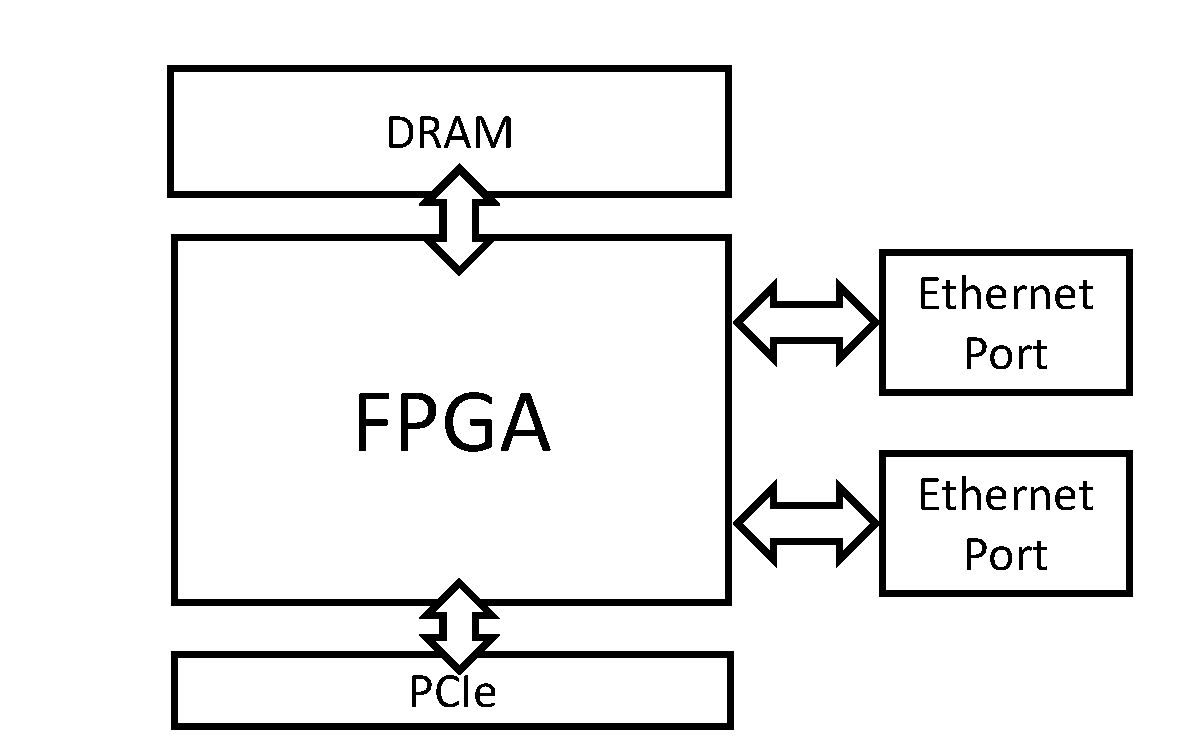
\includegraphics[width=0.3\textwidth]{fpga-board.pdf}
\vspace{-10pt}
\caption{A logic diagram of a FPGA board.}
\label{fig:fpga}
\vspace{-10pt}
\end{figure}

%
% we need to make more points here: parallelism, memory hierarchy, or code?
%

% setup the context of fpga parallelism
Compared to CPU or GPU, FPGAs usually have a much lower clock frequency
and a smaller memory bandwidth.
For example, typical clock frequency of a FPGA is about 200MHz, 
more than an order of magnitude slower than CPU (at 2\approx 3~GHz). 
Similarly, the bandwidth to a single Block memory or external DRAM of FPGA 
is usually 2\approx 10~GBps, while the memory bandwidth
is about 40~GBps of Intel XEON CPU and 100~GBps for a GPU. 
%
However, the CPU or GPU have only limited cores, which limits parallelism.
FPGAs have a massive amount of parallelism built-in. 
Modern FPGAs may have millions of LEs, hundreds K-bit registers, tens of M-bits of BRAM, 
and thousands 
of DSP blocks. In theory, each of them can work in parallel. 
Therefore, there could be thousands of parallel ``\textit{cores}'' 
running simultaneously inside a FPGA chip. 
Although the bandwidth of a single BRAM may be limited, if we access the  
thousands of BRAMs in parallel, the aggregate memory bandwidth can be multiple TBps! 
%
Therefore, to achieve high performance, a programmer
must fully utilize this massive parallelism.

% lead back to programming
Conventionally, FPGAs are programmed using HDLs like Verilog and VHDL.
These languages are too low level, hard to learn and complex to program.
As a consequence, the large community of software programmers has stayed away from FPGA for years~\cite{bacon2013fpga}. 
To ease this, many high level synthesis (HLS) 
tools/systems have been developed in
both industry and academia that try to convert a program in high level
language (predominately C) into HDLs. 
However, as we will show in the next subsection, none of them is 
suitable for network function processing, which is the focus of this work.


\subsection{Programming FPGA for NFs}

Our goal is to build a versatile, high performance network function 
platform with FPGA-acceleration. Such a platform should satisfy 
the following requirements.

\smalltitle{Flexibility.} The platform should be 
\textit{fully programmed using high-level languages.} 
Developers program with high-level abstractions and familiar tools, and
have similar programming experience as if programming on a multi-core processor.
We believe this is a necessary condition for FPGA to be accessible to
most software programmers.

\smalltitle{Modularized.} We should support a \textit{modular architecture}
for packet processing. Previous experiences on virtualized NFs
have demonstrated that a right modular architecture can well capture many common 
functionalities in packet processing~\cite{kohler2000click,martins2014clickos},
making them easy to reuse in various NFs.

\smalltitle{High performance and low latency.} NFs in datacenters
should handle a large amount of packets flowing at the line-rates of 40/100~Gbps
with ultra-low latency. Previous work has shown~\cite{rollback-mb} that even a few
hundred microseconds of latency added by NFs would have 
negative impacts on service experience.

\smalltitle{Support joint CPU/FPGA packet processing.} We'd say FPGA is no panacea. 
As inferred from the FPGA architecture discussed earlier in \S\ref{subsec:fpga}, not all tasks are 
suitable for FPGA. For example, algorithms that are naturally sequential and
processing that has very large memory footprint with low locality, should process  
better in CPU.
Additionally, FPGA has a strict area constraint. 
That means you cannot fit an arbitrarily large logic into a chip.
Dynamically swapping FPGA configurations without data plane interruption
is very difficult, as the reconfiguration time may take
seconds to minutes, depending on the FPGA's size.
%
Therefore, we should support fine-grained processing 
separation between CPU and FPGA. This requires high-performance communication 
between CPU and FPGA.


No of existing high level programming tools for FPGA satisfy all aforementioned requirements.
% HLS
Most HLS tools, \eg, Vivado HLS~\cite{vivado}, are only auxiliary tools 
for HDL tool chains. 
Instead of directly compiling a program into FPGA images, these tools generate only hardware 
modules, \ie, IP cores, which must be manually embedded in a HDL project and connected to other HDL modules
-- a mission impossible for most software programmers. 

% OpenCL
Altera OpenCL, however, may directly compile an OpenCL program to FPGA~\cite{aoc}. 
However, the OpenCL programming model is directly derived from GPU programming and 
is not modularized for packet processing. 
%
Further, OpenCL does not support joint packet processing between CPU and FPGA very well:
%
First, communication between a host program and a kernel in FPGA must always go through the onboard DDR memory. This adds non-trivial latency
and also causes the on-board memory a bottleneck.
%
Second, OpenCL kernel functions are \textit{called} from the host program. 
Before a kernel terminates, the host program cannot control the kernel behavior, \eg setting new parameters, nor reading any kernel state. 
But NFs face a continuous stream of packets and should be always running.

Click2NetFPGA~\cite{Click2NetFPGA} provides a modular architecture by 
directly compiling a Click modular router~\cite{kohler2000click} program into FPGA.
%
However, the performance of \cite{Click2NetFPGA} is much lower (two orders of magnitude) than what we report in this paper, as there are several bottlenecks in their system design (\eg, memory and packet I/O) and they also miss 
several important
optimizations to ensure fully pipelined processing (as discussed in~\S\ref{sec:optimization}). 
Additionally, \cite{Click2NetFPGA} does not support FPGA/CPU joint processing and thus unable to update configuration or read states while data plane is running.


In the following, we will present \name, a novel FPGA-accelerated 
network function platform that satisfies all aforementioned four requirements.


\egg{
Today's data centers rely on a wide range of network functions to implement network virtualization, ensure security (e.g. firewalls and intrusion detection/prevention systems), perform measurements and improve performance (e.g. traffic scheduling). As data centers are moving towards 40 Gbps bandwidth at end hosts, where the line-rate is 60 M packets per second for minimum-sized packets, higher throughput requirement is imposed upon network processors. Furthermore, as data center services are evolving rapidly, programmability becomes indispensable for network processors. However, existing network processors has a large mismatch to the performance and programmability requirements.

\subsection{Architectures for Network Processors}

Network processors based on general-purpose CPUs such as ClickOS \cite{martins2014clickos} enjoy good programmablity, modularity and composabilty, but the packet forwarding performance of a single core could not keep up with 10 Gbps line rate for minimum-sized packets, even before any network function is plugged in. Because CPU instructions are executed one-by-one and have low parallelism, packet processing performance would drop further as more network functions are added. If a CPU-based network processor is added bump-in-the-wire, there will be 10s of microseconds additional end-to-end latency \cite{martins2014clickos} which is one magnitude higher than the switching fabric. In network virtualization scenario, if packet encapsulation and decapsulation is done at end hosts, as in the case of virtual switch, NIC offloading mechanisms including Large Send Offload (LSO) and Large Receive Offload (LRO) have to be disabled, which has a huge impact on TCP performance \cite{yoshino2008performance}.

ASICs are known to be high-performance, but the network functions are fixed. Commodity switching ASICs typically have a pipeline of network functions \cite{broadcomethernet}, where each function can be configured via registers and a match table based on TCAM or memory. Some ASICs provide flexible OpenFlow-like match-action tables \cite{broadcomopenflow}, but the packet parser is fixed (we could not support new packet header and shim layer formats), actions are not extensible and the order of network functions in the pipeline is not reconfigurable.

GPUs are widely used as co-processors for computing-intensive tasks, but its SIMD (Single-Instruction Multiple-Data) programming model does not fit network processing, where different types of packets may take various execution flows. The high power consumption, high latency of batch processing and inability to receive and send network packets without CPU intervention are also factors that render GPU-based network processor infeasible in data centers.

Fortunately, reconfigurable hardware is an architecture that provides both programmability, high performance and power efficiency for certain workloads. FPGA (field programmable gate arrays) is the most prominent example of reconfigurable hardware. FPGAs can implement arbitrary logic function and utilize distributed on-chip registers and SRAM to exploit bit-level and task-level parallelism, therefore stream processing pipelines would not ``hit the memory wall'' as in Von Neumann architecture \cite{bacon2013fpga}. FPGA has shown potential in accelerating many workloads in cloud \cite{putnam2014reconfigurable}. Moreover, Moore's law is still working in FPGA industry, because the fabrication technology of FPGA is currently several generations behind the CPU industry [citation required].

\subsection{FPGA Programming Challenge}

Despite FPGA's potential in network processing, the programmablity of FPGA is traditionally provided by hardware description languages (HDL) such as Verilog, which requires hardware knowledge and are much harder to program and debug than higher-level languages such as C/C++. Thus, existing FPGA-based network processors such as NetFPGA \cite{lockwood2007netfpga} are hard to program for software engineers.

Many works, e.g. OpenFlow \cite{mckeown2008openflow}, P4 \cite{bosshart2014p4} and SDNet \cite{xilinxsdnet}, provides the programmability by abstracting a set of primitives in network processing and defining a high-level programming language to compose the primitives. This direction has proved effective, but the programmability is limited to a set of pre-defined actions, which could not keep pace with rapid development of data center network functions. Our work strive to make the primitives extensible for software engineers.

Fortunately, several frameworks have been proposed to provide abstractions for generic FPGA programming. Examples of such works include Xilinx Vivado HLS (High Level Synthesis) \cite{feist2012vivado} based on C/C++, Altera SDK for OpenCL \cite{czajkowski2012opencl} based on C-like OpenCL and IBM Lime \cite{auerbach2010lime} based on Java.

However, FPGA has a completely different architecture than general-purpose CPUs. For software programmers that bear Von Neumann model in mind, the compilers may generate surprisingly poor hardware logic for reasonable code in high-level language. For example, Click2NetFPGA \cite{Click2NetFPGA} uses LLVM and HLS tools to compile optimized Click C++ code into HDL, but the resulting FPGA-based router can only process 178 K pps (packets per second) for 98B packets, and 215 Mbps for large packets, which is 30 -- 50x slower than a CPU core in ClickOS \cite{martins2014clickos}. The bottleneck for small packets is the IP header checking stage \cite{Click2NetFPGA} because this stage is not fully pipelined; the bottleneck for large packets is the byte-wide shared memory \cite{Click2NetFPGA}, indicating a shared-memory design suitable for Von Neumann model would yield poor performance on FPGA.

FPGA has millions of logic gates with 10x slower clock rate than CPU, thousands of distributed fast SRAMs each with only KB capacity, and a large DRAM with 10x lower throughput than DRAMs in CPU architecture. Consequently, exploiting both spatial and temporal parallelism is crucial to unleashing the performance of FPGA. In network stream processing, most operations are independent of each other and therefore can be either parallelized (spatial) or pipelined (temporal), so that each stage of the pipeline can process different packets in parallel.

\subsection{Design Goals}
\label{subsec:designgoals}

We highlight several design goals for our ClickNP framework to enable software engineers to write efficient network applications.

\smalltitle{Modularity.} Modularity is one key feature that improves parallelism, since modules do not have shared state and can run in parallel by nature. Borrowing the concepts from Click modular router \cite{kohler2000click}, \textit{elements} are basic building blocks of network functions. Elements run asynchronously and are connected via uni-directional \textit{channels}. The network processing pipeline is a data flow graph of elements and channels, starting from Ethernet receivers and ending at Ethernet transmitters.

\smalltitle{Line-rate throughput.} To allow efficient processing of packet content, an Ethernet packet is split into 32-byte \textit{flits} before feeding into elements. In the worst case, when 69-byte packets are received back-to-back, the line rate would be 40G / 8 / (69+20) = 56.18 Mpps, which splits into 56.18M * 3 = 168.54M flits. Every clock cycle an element reads at most one flit and outputs zero or one flit. This means any FPGA pipeline with clock frequency lower than 168.54 MHz would not be able to achieve line rate. If we waste a cycle between every two packets, the minimum clock frequency would be 224.72 MHz. However, on Stratix V FPGA platform \cite{stratix2012device}, non-trivial hardware logic that accesses registers and local memory can hardly run higher than 200 MHz. Therefore no idle cycles are allowed in elements processing packet content. First, the framework should provide abstractions for programmers to develop fully pipelined network functions. Second, as full compilation of a FPGA program may take hours, the framework should give performance warnings in an early compilation stage if the code cannot be fully pipelined.

\smalltitle{Code reuse.} Many network applications share a common set of elements, for example packet parser, lookup tables and packet modifications. Code of these elements should be reusable and elements should be composable. Software engineers should be able to write many network applications simply by connecting elements in the library.

\smalltitle{Debugging support.} First, as HDL (e.g. Verilog) simulation and debugging is both time consuming and requires extensive hardware knowledge, the framework should be able to compile OpenCL-based ClickNP programs to native x86 code for emulation, and provide traffic generators and receivers to test functionality. Second, as CPU is neither capable of sending or receiving packets at 60 Mpps, we need a FPGA-based network benchmark suite to perform stress testing on the network processor.

\smalltitle{Separation of control plane and data plane.} On one hand, our throughput requirement requires most network packets to be processed through the reconfigurable hardware without any CPU intervention. On the other hand, SDN and NFV applications are usually complicated and have external dependencies. Therefore a clear interface between the control plane and the data plane is mandatory, where data plane programs are written within ClickNP framework and target massive parallelism, and control plane programs need only slight modifications to call our host library and perform on-the-fly reconfigurations.

\smalltitle{Host communication.} Network processors require low-latency and high-throughput interactions with the host machine. In SDN and NFV applications, FPGA needs to send unknown packets to the controller and request a new forwarding rule to be inserted into FPGA. The round-trip time should be as low as possible to reduce end-to-end flow establish time. In packet replay and capture applications, FPGA needs to receive or send Gigabytes of packets from or to the host machine without using the network adapter.

We design ClickNP to meet the above design goals with Catapult FPGA \cite{putnam2014reconfigurable} and Altera OpenCL \cite{singh2011implementing}. In the next section, we will describe the FPGA and OpenCL components, and how we build a toolchain that abstracts away hardware specific details.
}

\egg{
\subsection{FPGA in datacenter}

Conventionally, datacenter operators largely relied on the performance improvements in general-purpose servers
to improve the operation efficiency. This performance improvement rate of servers 
has considerably slowed down recently due to the power limitations~\cite{putnam2014reconfigurable, more-citation}.
This has motivated the adoption of \textit{accelerator} that can be specialized to certain workloads to get efficiency gains.
However, the non-programmable ASIC-based accelerators are undesirable for datacenters due to following two reasons:
Firstly, datacenter operators prefers homogeneous server configurations to minimize the management overhead and also provide
a consistent platform that applications can rely on.
Secondly, services in datacenters evolve extremely rapidly. Waiting for the long release cycle of ASIC chips is undesirable.
%
Therefore, it requires a flexible accelerator that can potentially speed up many applications.
%
GPU and FPGA are two predominate technologies that satisfy this requirement.

% comparison between GPU and FPGA
% power efficiency
Compared with GPU, FPGA is more power efficient. For example, the latest NIVDIA xxx consumes xxx W power, while a high-end
Altera Stratix V consumes xxx W power ( J per op?) \knote{need a citation}. 
% versatile 
Further, FPGA is more versatile. While GPU is mainly designed to achieve \textit{data parallelism} with SPMD (single program, multiple data), 
FPGA can easily achieve both data parallelism and \textit{task parallelism} as different block of LEs can be independently configured to
implement different processing.  
% I/O
Finally, FPGA supports various I/O interface. Normally, GPU can only communicate with PC memory through PCIE bus. 
But FPGA can input or output data from many interfaces like network ports, and is more suitable for processing these 
I/O streams. 

FPGA is a mature technology and becomes inexpensive. A large scale deployment of FPGA in Microsoft datacenter shows 
that a high-end FPGA board increases the total cost of ownership (TCO) of a server by less than 30\%, but can double 
the Bing search efficiency~\cite{putnam2014reconfigurable}.
%
In this paper, we focus on using FPGA to accelerate network functions that are essential to our datacenter networks.
}

\egg{
\smalltitle{inexpensive}

Why I need this as background:
\begin{itemize}
\item Price issue?
\item Power?
\item Transition to FPGA for network functions?
\end{itemize}
}
